\documentclass[12pt, dvipdfmx]{article}
\usepackage[margin=1in]{geometry}
\usepackage{enumitem}
\usepackage{amsmath}
\usepackage{bm}
\usepackage{graphicx}

\title{
  \vspace{-2cm}
  CS 224n Assignment \#2 \\
  \author{Yoshihiro Kumazawa}
}

\begin{document}
\maketitle
\begin{enumerate}[label=\textbf{\arabic*}]
  \item \textbf{Written}
  \begin{enumerate}[label=(\alph*)]
    \item \[-\sum_{w\in Vocab}y_w\log(\hat{y}_w)=\sum_{w=o}\log(\hat{y}_w)=\log(\hat{y}_o).\]
    \item
    \begin{align*}
      \frac{\partial}{\partial\bm{v}_c}\bm{J}_{\textrm{naive-softmax}}(\bm{v}_c,o,\bm{U}) &=\frac{\partial}{\partial\bm{v}_c}\left(-\log\left(\frac{\exp(\bm{u}_o^\top\bm{v}_c)}{\sum_{w\in Vocab}\exp(\bm{u}_w^\top\bm{v}_c)}\right)\right) \\
      &=\frac{\partial}{\partial\bm{v}_c}\left(\log\left(\sum_{w\in Vocab}\exp(\bm{u}_w^\top\bm{v}_c)\right)-\log\left(\exp(\bm{u}_o^\top\bm{v}_c)\right)\right) \\
      &=\frac{\partial}{\partial\bm{v}_c}\log\left(\sum_{w\in Vocab}\exp(\bm{u}_w^\top\bm{v}_c)\right)-\frac{\partial}{\partial\bm{v}_c}\bm{u}_o^\top\bm{v}_c \\
      &=\frac{\sum_{x\in Vocab}\exp(\bm{u}_x^\top\bm{v}_c)\bm{u}_x}{\sum_{w\in Vocab}\exp(\bm{u}_w^\top\bm{v}_c)}-\bm{u}_o \\
      &=\sum_{x\in Vocab}\frac{\exp(\bm{u}_x^\top\bm{v}_c)}{\sum_{w\in Vocab}\exp(\bm{u}_w^\top\bm{v}_c)}\bm{u}_x-\bm{u}_o \\
      &=\sum_{x\in Vocab}\bm{\hat{y}}_x\bm{u}_x-\sum_{x\in Vocab}\bm{y}_x\bm{u}_x \\
      &=\sum_{x\in Vocab}\bm{u}_x(\bm{\hat{y}}_x-\bm{y}_x) \\
      &=\bm{U}(\bm{\hat{y}}-\bm{y}).
    \end{align*}
    \item
    \begin{align*}
      \frac{\partial}{\partial\bm{u}_w}\bm{J}_{\textrm{naive-softmax}}(\bm{v}_c,o,\bm{U}) &=\frac{\partial}{\partial\bm{u}_w}\log\left(\sum_{w\in Vocab}\exp(\bm{u}_w^\top\bm{v}_c)\right)-\frac{\partial}{\partial\bm{u}_w}\bm{u}_o^\top\bm{v}_c \\
      &=\frac{\exp(\bm{u}_w^\top\bm{v}_c)}{\sum_{w\in Vocab}\exp(\bm{u}_w^\top\bm{v}_c)}\bm{v}_c-\bm{y}_w\bm{v}_c \\
      &=\bm{\hat{y}}_w\bm{v}_c-\bm{y}_w\bm{v}_c \\
      &=\bm{v}_c(\bm{\hat{y}}_w-\bm{y}_w).
    \end{align*}
    \item \[\frac{d}{d\bm{x}}\sigma(\bm{x})=\frac{d}{d\bm{x}}\frac{1}{1+e^{-\bm{x}}}=\frac{e^{-\bm{x}}}{(1+e^{-\bm{x}})^2}=\sigma(\bm{x})(1-\sigma(\bm{x})).\]
    \item
    \begin{align*}
      \frac{\partial}{\partial\bm{v}_c}\bm{J}_{\textrm{neg-sample}}(\bm{v}_c,o,\bm{U}) &=\frac{\partial}{\partial\bm{v}_c}\left(-\log(\sigma(\bm{u}_o^\top\bm{v}_c))-\sum_{k=1}^K\log(\sigma(-\bm{u}_k^\top\bm{v}_c))\right) \\
      &=-\frac{\partial}{\partial\bm{v}_c}\log(\sigma(\bm{u}_o^\top\bm{v}_c))-\sum_{k=1}^K\frac{\partial}{\partial\bm{v}_c}\log(1-\sigma(\bm{u}_k^\top\bm{v}_c)) \\
      &=-\frac{\sigma(\bm{u}_o^\top\bm{v}_c)(1-\sigma(\bm{u}_o^\top\bm{v}_c))}{\sigma(\bm{u}_o^\top\bm{v}_c)}\bm{u}_o+\sum_{k=1}^K\frac{(1-\sigma(\bm{u}_k^\top\bm{v}_c))\sigma(\bm{u}_k^\top\bm{v}_c)}{1-\sigma(\bm{u}_k^\top\bm{v}_c)}\bm{u}_k \\
      &=-(1-\sigma(\bm{u}_o^\top\bm{v}_c))\bm{u}_o+\sum_{k=1}^K\sigma(\bm{u}_k^\top\bm{v}_c)\bm{u}_k. \\
      \frac{\partial}{\partial\bm{u}_o}\bm{J}_{\textrm{neg-sample}}(\bm{v}_c,o,\bm{U}) &=-\frac{\partial}{\partial\bm{u}_o}\log(\sigma(\bm{u}_o^\top\bm{v}_c))=-(1-\sigma(\bm{u}_o^\top\bm{v}_c))\bm{v}_c.\\
      \frac{\partial}{\partial\bm{u}_k}\bm{J}_{\textrm{neg-sample}}(\bm{v}_c,o,\bm{U}) &=-\frac{\partial}{\partial\bm{u}_k}\sum_{k=1}^K\log(1-\sigma(\bm{u}_k^\top\bm{v}_c))=\sigma(\bm{u}_k^\top\bm{v}_c)\bm{v}_c.
    \end{align*}
    These are computationally less expensive than the naive-softmax loss because its summation ranges over only $K$ numbers, which is usually much smaller than $|Vocab|$.
    \item
    \begin{enumerate}[label=(\roman*)]
      \item $\partial\bm{J}_{\textrm{skip-gram}}(\bm{v}_c,w_{t-m},\ldots,w_{t+m},\bm{U})/\partial\bm{U}=\sum\limits_{\substack{-m\leq j\leq m\\j\neq 0}}\partial\bm{J}(\bm{v}_c,w_{t+j},\bm{U})/\partial\bm{U}.$
      \item $\partial\bm{J}_{\textrm{skip-gram}}(\bm{v}_c,w_{t-m},\ldots,w_{t+m},\bm{U})/\partial\bm{v}_c=\sum\limits_{\substack{-m\leq j\leq m\\j\neq 0}}\partial\bm{J}(\bm{v}_c,w_{t+j},\bm{U})/\partial\bm{v}_c.$
      \item $\partial\bm{J}_{\textrm{skip-gram}}(\bm{v}_c,w_{t-m},\ldots,w_{t+m},\bm{U})/\partial\bm{v}_w=0.$
    \end{enumerate}
  \end{enumerate}
  \item \textbf{Coding}
  \begin{enumerate}[label=(\alph*)]
    \item See \texttt{word2vec.py}.
    \item See \texttt{sgd.py}.
    \item
    \begin{figure}
      \centering
      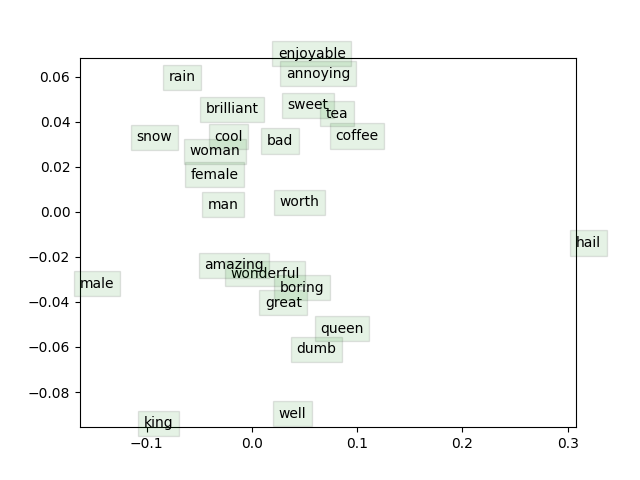
\includegraphics{../word_vectors.png}
      \caption{Visualized word vectors}
      \label{fig:word_vectors}
    \end{figure}
    Figure~\ref{fig:word_vectors} shows the visualized word vectors. Some similar words like 'woman' and 'female' are put close but other similar words like 'man' and 'male' are far apart. Thus our word embedding does not retain the parallelogram property that well-trained word embedding methods are expected to have.
  \end{enumerate}
\end{enumerate}
\end{document}
